\section{Bridging The Corpora}
\label{sec:bridging}

\newcommand{\nBlueprintPairs}{1{,}595\xspace}
\newcommand{\nBlueprintFormal}{1{,}577\xspace}
\newcommand{\nBlueprintInformal}{1{,}308\xspace}
\newcommand{\nSwept}{385{,}657\xspace}
\newcommand{\pctCandidate}{55.3\%\xspace}
\newcommand{\nJudged}{100{,}799\xspace}
\newcommand{\matchTotal}{47{,}952\xspace}
\newcommand{\matchRateAll}{48\%\xspace}
\newcommand{\rateNinety}{87\%\xspace}
\newcommand{\nNinety}{6{,}353\xspace}
\newcommand{\yieldSeventy}{23\%\xspace}
\newcommand{\yieldSixty}{2\%\xspace}
\newcommand{\dsMatch}{61{,}234\xspace}
\newcommand{\dsRate}{61\%\xspace}

\paragraph{Motivation.} To bridge the formal and informal graphs into a Universal Graph, we look for \textbf{matches}: (informal, formal) statement pairs that express the same mathematical result under the same assumptions. A Lean blueprint~\citep{massot2020leanblueprint} is a \LaTeX{} document that writes out a development's definitions, statements, and proofs in human-readable form, and links each statement to the Lean declaration that formalizes it through author-written \texttt{\textbackslash lean\{\}} annotations. These links give us a small set of such matches\footnote{\nBlueprintPairs{} (informal, formal) statement pairs drawn from blueprints, across \nBlueprintInformal{} informal statements and \nBlueprintFormal{} formal declarations; one informal statement is often formalized as several Lean lemmas, which is why formals outnumber informals.}. Extending this set and finding such links at scale better connects Lean to the informal mathematics it formalizes, and gives neural theorem provers and auto-formalization systems an accurate scaffold by which new formalizations can come about.

\paragraph{Setup.} Our matching pipeline (Figure~\ref{fig:pipeline}) searches from the smaller, lightly-filtered\footnote{We drop constructors (\texttt{ctor}) and compiler-internal auto-generated names, which lack a meaningful natural-language counterpart. This amounts to 2{,}448 nodes ($0.63\%$) and leaves the \nBlueprintPairs{} blueprint pairs intact.} formal graph of \nSwept{} declarations into the informal corpus. For each formal declaration we embed its natural-language slogan and retrieve the single most similar informal slogan by cosine similarity; that nearest neighbor, with its similarity score, is a \textbf{candidate match}.\footnote{Both graphs are embedded into one shared index, so this is a cross-modal nearest-neighbor query, not a per-side search.} At \texttt{ann\_k=50} this finds a candidate for \pctCandidate{} of declarations and yields the similarity distribution in Table~\ref{tab:sim-bins}.

Modulating \texttt{ann\_k} between $500$ and $1000$ over a sample of $200$ otherwise-unmatched declarations, we see that deeper search does recover a candidate for $84\%$ and $88\%$ of them respectively, but only up to a similarity of $0.837$ and $0.859$. Across all $400$ of these deeper probes only a single candidate clears the $0.85$ match bar and none reach $0.90$, so a missing candidate at \texttt{ann\_k=50} almost always reflects the genuine absence of a close informal counterpart rather than a search-horizon limitation.

\definecolor{soft}{HTML}{EAF0F8} 

\begin{table}[t]\centering\small\setlength{\tabcolsep}{6pt}
    \begin{tabular}{@{}l r@{}}\toprule
    Similarity bin & Decls. \\\midrule
    \rowcolor{soft}0.95--1.0  & 678 \\
    \rowcolor{soft}0.90--0.95 & 6{,}636 \\
    \rowcolor{soft}0.85--0.90 & 26{,}807 \\
    \rowcolor{soft}0.80--0.85 & 66{,}744 \\
    0.50\textsuperscript{*}--0.80 & 112{,}481 \\
    no match  & 172{,}311 \\\midrule
    Total      & 385{,}657 \\\bottomrule
    \end{tabular}
    \caption{\textbf{Candidate match} cosine similarity across all 385,657 swept formal declarations. Shaded rows are the tiers evaluated using LLM-as-judge. 0.50* is the minimum retrieved similarity and no match represents declarations with no informal neighbor at \texttt{ann\_k=50}.}
    \label{tab:sim-bins}
\end{table}

\begin{figure*}[t]\centering
    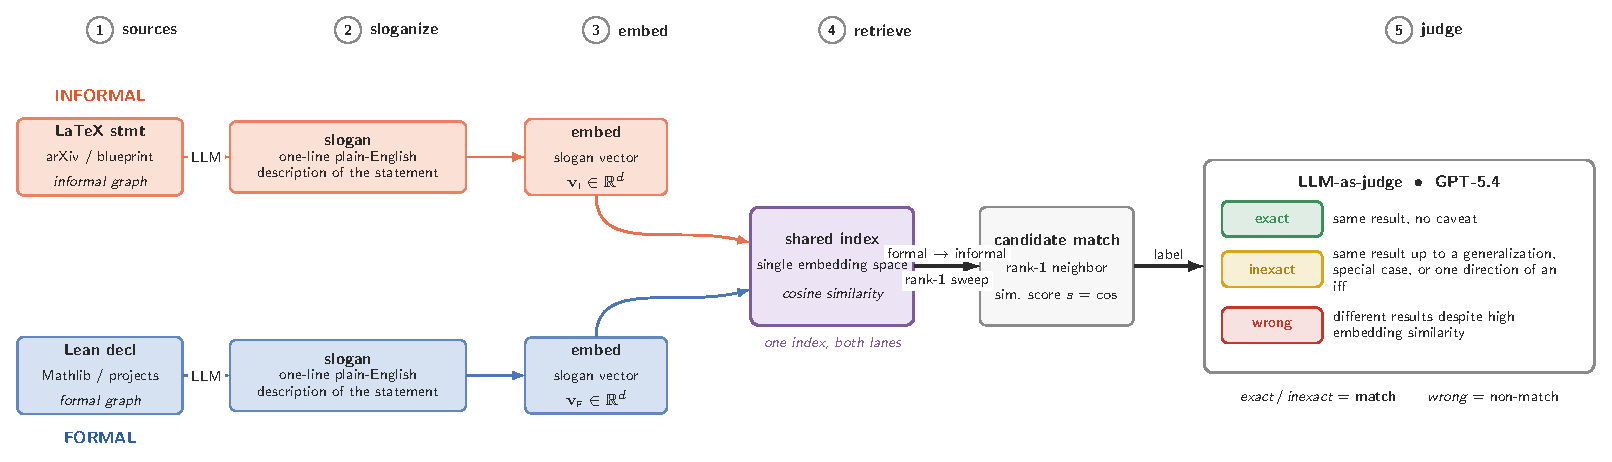
\includegraphics[width=\textwidth]{matching_pipeline_v3.pdf}
    \caption{The matching pipeline. Lean declarations and \LaTeX{} statements are each
    sloganized and embedded into one shared index; a formal$\to$informal rank-1 cosine query
    proposes candidate matches, which a single GPT-5.4 judge labels \texttt{exact} /
    \texttt{inexact} / \texttt{wrong} (\texttt{exact}/\texttt{inexact} count as matches).}
    \label{fig:pipeline}
\end{figure*}

\paragraph{Does retrieval find true counterparts?} Embedding formal and informal slogans into one shared space is what makes cross-modal matching possible: a formal statement can be paired with its informal counterpart directly by embedding similarity, with no shared vocabulary or surface overlap required. We validate that this similarity actually recovers true counterparts using blueprint pairs as a source of truth, where each blueprint annotates a Lean declaration with a human-written informal statement. The informal halves sit in our corpus like any other slogan (labeled \texttt{source=blueprint}), with the same embeddings and none treated specially.

We take each blueprint's \emph{formal} slogan as the query and ask which informal slogan is most similar to it in the shared index, then check where the annotated informal partner lands in that ranking. The partner ranks first 43.5\% of the time and within the top ten 69.9\% (Hit@1, Hit@10). Mismatches with the annotated partner are mostly not errors: among formal nodes whose top result is \emph{not} the annotated partner but is itself a high-similarity candidate ($\geq 0.85$), LLM-as-judge rates 65\% (n=187) as matches, i.e.\ valid alternative restatements rather than retrieval failures.

\paragraph{Judging.} To judge matches, a GPT-5.4 judge labels each candidate, given the declaration name, both slogans, the Lean signature, the arXiv title, and the informal \LaTeX. The judge returns its decision as one label with a brief rationale:
\begin{itemize}
\setlength{\itemsep}{1pt}
\item \bx{green!20}{\texttt{exact}}: the same result without caveat; a mathematician could cite one as the other.
\item \bx{yellow!35}{\texttt{inexact}}: the same underlying result but not verbatim (a generalization, special case, or one direction of a bidirectional implication).
\item \bx{red!22}{\texttt{wrong}}: different results despite high embedding similarity (shared vocabulary or sibling concepts).
\end{itemize}
We count \texttt{exact} and \texttt{inexact} as matches. GPT-5.4 is our judge of record because it is stricter than our initial choice, Opus~4.8, which a domain expert found over-generous; since a curated set should favor precision, we adopt the stricter judge (selection and an expert re-grading are in Appendix~\ref{app:calib}). The judge is stable under re-runs: a second independent GPT-5.4 pass over a random 500-candidate sample agrees on the match/non-match verdict for $93.2\%$ of pairs ($\kappa{=}0.86$)\footnote{Cohen's $\kappa$ corrects agreement for chance: $\kappa = (p_o - p_e)/(1 - p_e)$, where $p_o$ is the observed agreement and $p_e$ the agreement expected if the two raters labeled independently at their observed match rates.}, so re-running GPT-5.4 rarely changes a verdict.

\paragraph{Where to judge.} We judge every candidate at cosine similarity $0.8$ and above. We set the floor here, rather than higher, to make the curated set as valuable as possible: it captures the broad band of \texttt{inexact} matches alongside the \texttt{exact} ones, and because each edge is stored with its deterministic graph context, later work can re-judge these looser links with more information and promote \texttt{inexact} ties to \texttt{exact}. We do not go lower because the \textbf{yield rate} (the fraction the judge affirms as a match) collapses below $0.8$: a pilot of 150 candidates per $0.1$-wide bin confirms only \yieldSeventy{} in $0.7$--$0.8$ and \yieldSixty{} in $0.6$--$0.7$, where judging mostly confirms non-matches. Above the floor the match rate climbs steeply with similarity (Figure~\ref{fig:comp}).

\paragraph{Judged matches.} Of the \nJudged{} candidates above the floor\footnote{The retrieval pool holds 100{,}865 candidates at similarity $\geq 0.8$ (Table~\ref{tab:sim-bins}); 100{,}831 were submitted to GPT-5.4 and 32 returned unparseable output, giving these 100{,}799 valid labels. Of them, 187 are \texttt{unjudgeable}, leaving 100{,}612 with a decisive \texttt{exact}/\texttt{inexact}/\texttt{wrong} verdict.}, GPT-5.4 affirms \matchTotal{} as matches (\matchRateAll). Quality concentrates at the high-similarity end: the $\geq\!0.9$ tier alone gives \nNinety{} matches (\rateNinety{} of its candidates), and the affirmation rate rises steadily with similarity across the band (Figure~\ref{fig:comp}). Running a second, more lenient judge (DeepSeek-V4-Pro) over the same candidates affirms \dsMatch{} (\dsRate); we keep the stricter GPT-5.4 set as our matches and report DeepSeek as a high-recall comparison.

\begin{figure*}[t]
  \centering
  \begin{subfigure}{0.49\linewidth}
    \centering
    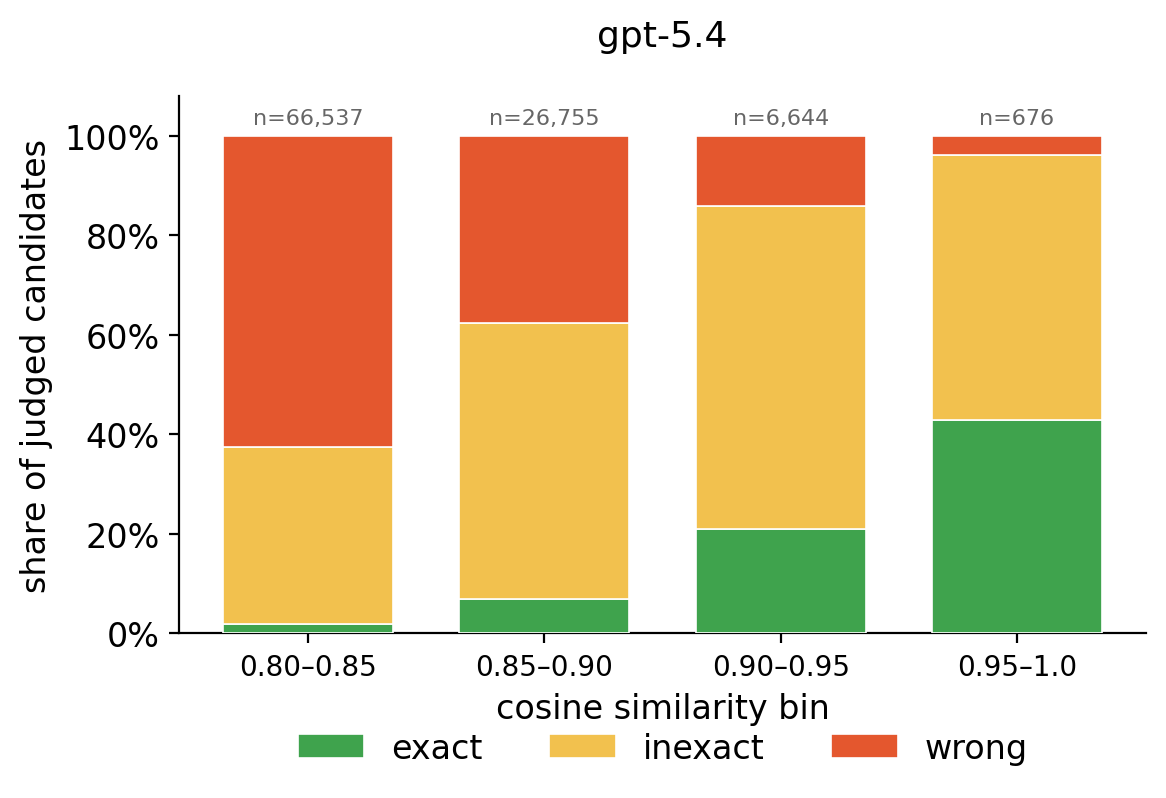
\includegraphics[width=\linewidth]{verdict_composition_g54.png}
    \caption{GPT-5.4, our judge of record.}
    \label{fig:comp-g54}
  \end{subfigure}
  \hfill
  \begin{subfigure}{0.49\linewidth}
    \centering
    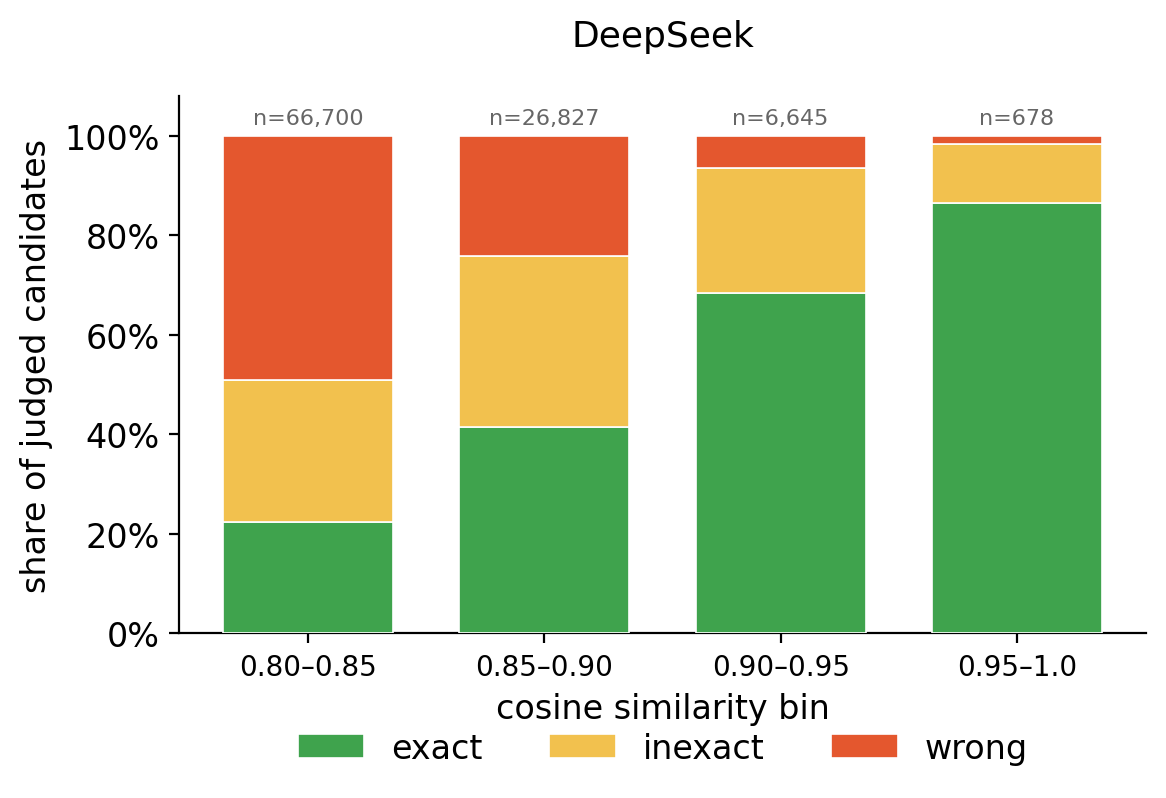
\includegraphics[width=\linewidth]{verdict_composition_deepseek.png}
    \caption{DeepSeek, a more lenient high-recall comparison.}
    \label{fig:comp-ds}
  \end{subfigure}
  \caption{Verdict composition by cosine-similarity bin (candidates at $\geq\!0.8$). Both judges shift from \texttt{wrong} to \texttt{exact} and \texttt{inexact} as similarity rises; DeepSeek is consistently more generous, so we keep GPT-5.4 as the stricter set of record and report DeepSeek as a high-recall comparison.}
  \label{fig:comp}
\end{figure*}

\paragraph{Looking to the future.} Embedding both graphs into one space turns cosine similarity into a signal of ``warmth'' that curates high-quality links across two large and largely disconnected bodies of mathematical writing. These links are hard to surface by hand yet cheap to check once proposed, and they give automated formalization systems concrete context to build on, speaking to the ``dependency issue'' Seed-Prover~1.5 describes, where progress ``typically hinges on synthesizing insights across a multitude of related papers''~\citep{chen2025seedprover15masteringundergraduatelevel}.